% Chapter 5 from the standard thesis template
%   with a full page figure and a sideways table.
\chapter{SUMMARY AND DISCUSSION}

This is the opening paragraph to my thesis which
explains in general terms the concepts and hypothesis
which will be used in my thesis.

With more general information given here than really
necessary.

\section{Introduction}

Here initial concepts and conditions are explained and
several hypothesis are mentioned in brief.

Or graphically as seen in \autoref{mgraph2}
it is certain that my hypothesis is true.

%\begin{figure}[p!] \centering

\begin{figure}[H] \centering % This goes with the package float comment this line out and use the previous one if you do not want to hold your position
    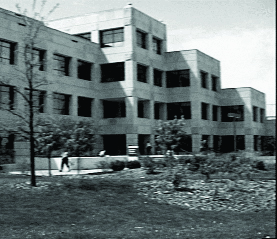
\includegraphics[alt={This is alt text}]{Images/dc5}

    \caption{Durham Centre---  Another View}
    \label{mgraph2}
\end{figure}

\subsection{Hypothesis}

Here one particular hypothesis is explained in depth
and is examined in the light of current literature.

As can be seen in \autoref{nothingelse} it is
truly obvious what I am saying is true.

%\addtocontents{lot}{\protect\newpage}
\begin{landscape}
    \hfill
    \vfill
    %h! necessary for it to be centered
    \begin{table}[h!] \centering
        \caption{This table shows almost nothing but is a
            sideways table and takes up a whole page by itself}
        \label{nothingelse}
        % Use: \begin{tabular{|lcc|} to put table in a box
        %\tagpdfsetup{table/header-rows={1,2}} would have rows 1 and 2 be header rows
        \tagpdfsetup{table/header-rows={1}}
        %Use \tagpdfsetup{table/header-columns={}} for header columns instead
        %Put \tagpdfsetup{table/multirow={⟨number of rows comma separated ⟩} in cells spanning multiple rows
        \begin{tabular}{lcc} \hline
            \textbf{Element} & \textbf{Control} & \textbf{Experimental} \\ \hline
            Moon Rings       & 1.23             & 3.38                  \\
            Moon Tides       & 2.26             & 3.12                  \\
            Moon Walk        & 3.33             & 9.29                  \\ \hline
        \end{tabular}
    \end{table}
    \hfill
    \vfill
\end{landscape}

\subsubsection{Parts of the hypothesis}

Here one particular part of the hypothesis that is
currently being explained is examined and particular
elements of that part are given careful scrutiny.

% Below \subsubsection
% Sectional commands: \paragraph and \subparagraph may also be used

%\addtocontents{toc}{\protect\newpage} %% Remove this if needed, this lines forces the lines of the TOC starting with the below sub-heading "Critical Review" to go to the next page. Remove this formatting line as it will be required only if you want to force a table of contents entry to the next page along with the other subsequent entries.

\subsection{Second Hypothesis}

Here one particular hypothesis is explained in depth
and is examined in the light of current literature.

\subsubsection{Parts of the second hypothesis}

Here one particular part of the hypothesis that is
currently being explained is examined and particular
elements of that part are given careful scrutiny.

\section{Criteria Review}

Here certain criteria are explained thus eventually
leading to a foregone conclusion.

\section{Results And Discussion}

Here the results can be inserted

